\documentclass{beamer}
\usetheme{Singapore}
\usepackage{changepage}

%\usepackage{pstricks,pst-node,pst-tree}
\usepackage{amssymb,latexsym}
\usepackage{tikz}
\usepackage{graphicx}
\usepackage{fancyvrb}
\usepackage{hyperref}
\usepackage{fancybox}
\usepackage[listings]{tcolorbox}

\definecolor{codegreen}{rgb}{0,0.6,0}
\definecolor{codegray}{rgb}{0.5,0.5,0.5}
\definecolor{codepurple}{rgb}{0.58,0,0.82}
\definecolor{backcolour}{rgb}{0.95,0.95,0.92}

\lstdefinestyle{mystyle}{
    language=Python,
    backgroundcolor=\color{backcolour},   
    commentstyle=\color{codegreen},
    keywordstyle=\color{magenta},
    numberstyle=\tiny\color{codegray},
    stringstyle=\color{codepurple},
    basicstyle=\ttfamily\footnotesize,
    breakatwhitespace=false,         
    breaklines=true,                 
    captionpos=b,                    
    keepspaces=true,                 
    numbers=left,                    
    numbersep=5pt,                  
    showspaces=false,                
    showstringspaces=false,
    showtabs=false,                  
    tabsize=2,
    escapechar=|,
    frame=single
}

\lstset{style=mystyle}


\newcommand{\bi}{\begin{itemize}}
\newcommand{\li}{\item}
\newcommand{\ei}{\end{itemize}}
\newcommand{\Show}[1]{
\begin{center}
\shadowbox{\begin{minipage}{0.8\textwidth}
          #1
          \end{minipage}}
\end{center}
}
\newcommand{\arrow}{\ensuremath{\rightarrow}}

\newcommand{\uparr}{\ensuremath{\uparrow}}


\newcommand{\fig}[2]{\centerline{\includegraphics[width=#1\textwidth]{#2}}}

\newcommand{\bfr}[1]{\begin{frame}[fragile]\frametitle{{ #1 }}}
\newcommand{\efr}{\end{frame}}

\newcommand{\cola}{\begin{columns}\begin{column}{0.5\textwidth}}
\newcommand{\colb}{\end{column}\begin{column}{0.5\textwidth}}
\newcommand{\colc}{\end{column}\end{columns}}


\title{Think Python 2e, Chapter 8 Notes}
\author{Geoffrey Matthews}

\begin{document}

\begin{frame}
\maketitle

\end{frame}

\bfr{Strings are sequences}

\centerline{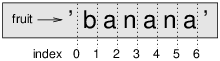
\includegraphics{thinkpython2009}}

\begin{lstlisting}
>>> fruit = 'banana'
>>> len(fruit)
6
>>> fruit[1]
'a'
>>> fruit[4]
'n'
>>> fruit[-1]
'a'
>>> fruit[1:3]
'an'
>>> fruit[2:]
'nana'
>>> fruit[:3]
'ban'
\end{lstlisting}

\end{frame}

\bfr{String traversal}
\begin{lstlisting}
index = 0
while index < len(fruit):
    letter = fruit[index]
    print(letter)
    index = index + 1
\end{lstlisting}
\begin{lstlisting}
for letter in fruit:
    print(letter)
\end{lstlisting}
\end{frame}


\bfr{Strings are immutable}
\begin{lstlisting}
>>> greeting = 'Hello, world!'
>>> greeting[0] = 'J'
TypeError: 'str' object does not support item assignment
\end{lstlisting}
\pause
You have to create a new string:
\begin{lstlisting}
>>> greeting = 'Hello, world!'
>>> new_greeting = 'J' + greeting[1:]
>>> new_greeting
'Jello, world!'
\end{lstlisting}

\end{frame}
\bfr{Searching}

\begin{lstlisting}
def find(word, letter):
    index = 0
    while index < len(word):
        if word[index] == letter:
            return index
        index = index + 1
    return -1
\end{lstlisting}

\end{frame}
\bfr{Looping and counting}

\begin{lstlisting}
word = 'banana'
count = 0
for letter in word:
    if letter == 'a':
        count = count + 1
print(count)
\end{lstlisting}

\end{frame}
\bfr{String methods}

\begin{lstlisting}
>>> word = 'banana'
>>> new_word = word.upper()
>>> new_word
'BANANA'
\end{lstlisting}

\begin{lstlisting}
>>> word = 'banana'
>>> index = word.find('a')
>>> index
1
>>> word.find('na')
2
>>> word.find('na', 3)
4
>>> name = 'boba'
>>> name.find('b', 1, 2)
-1
\end{lstlisting}


\end{frame}

\bfr{The {\tt in} operator}

\begin{lstlisting}
>>> 'nan' in 'banana'
True
>>> 'seed' in 'banana'
False
\end{lstlisting}

\begin{lstlisting}
def in_both(word1, word2):
    for letter in word1:
        if letter in word2:
            print(letter)
\end{lstlisting}

\begin{lstlisting}
>>> in_both('apples', 'oranges')
a
e
s
\end{lstlisting}

\end{frame}


\bfr{String comparison}

\begin{lstlisting}
if word == 'banana':
    print('All right, bananas.')
\end{lstlisting}

\begin{lstlisting}
if word < 'banana':
    print('Your word, '+word+', comes before banana.')
elif word > 'banana':
    print('Your word, '+word+', comes after banana.')
else:
    print('All right, bananas.')
\end{lstlisting}

\begin{lstlisting}
Your word, Pineapple, comes before banana.
\end{lstlisting}

Capital letters come before lowercase.

Solution: convert all to lowercase before comparison.

\end{frame}
\bfr{Vocabulary}
\begin{description}
\li[object:]
Something a variable can refer to. For now, you can use “object” and “value” interchangeably.
\li[sequence:]
An ordered collection of values where each value is identified by an integer index.
\li[item:]
One of the values in a sequence.
\li[index:]
An integer value used to select an item in a sequence, such as a character in a string. In Python indices start from 0.
\li[slice:]
A part of a string specified by a range of indices.
\li[empty string:]
A string with no ch]aracters and length 0, represented by two quotation marks.
\li[immutable:]
The property of a sequence whose items cannot be changed.
\end{description}
\end{frame}
\bfr{Vocabulary}
\begin{description}
\li[traverse:]
To iterate through the items in a sequence, performing a similar operation on each.
\li[search:]
A pattern of traversal that stops when it finds what it is looking for.
\li[counter:]
A variable used to count something, usually initialized to zero and then incremented.
\li[invocation:]
A statement that calls a method.
\li[optional argument:]
A function or method argument that is not required.


\end{description}
\end{frame}

\end{document}
